\documentclass{article}

\usepackage{tikz}

\begin{document}

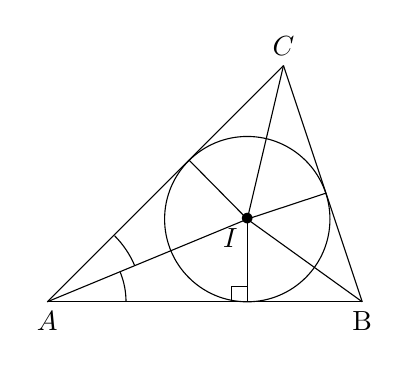
\begin{tikzpicture}
  % Triangle
  \draw (3,3)node[above]{$C$}  % C
      -- (4,0) node[below]{B}; % B
  \draw (0,0)node[below] {$A$} % A
      -- (3,3); 
  \draw (0,0)-- (4,0);
  % Cercle
  \draw(2.54,1.05) circle (1.05cm);
  % Rayons, projection de $I$
  \draw (1.8,1.8) % contact sur [AC]
      -- (2.54,1.05); 
  \draw (2.54,1.05) node[below left]{$I$} node{$\bullet$}
      -- (2.54,0); % contact sur [AB]
  \draw (2.54,1.05)
      -- (3.54,1.38); % contact sur [BC]
  % Bissectrices
  \draw (3,3)-- (2.54,1.05); % [IC]
  \draw (0,0)-- (2.54,1.05); % [IA]
  \draw (4,0)-- (2.54,1.05); % [IB]
  % marques d'angles
  \draw (1,0) arc(0:22:1); % (AB,AI)
  \draw (1.11,0.46) arc (23:45:1.2); % (AI,AC)
  % Angle droit sur [AB]
  \draw (2.34,0) -- (2.34,0.2) -- (2.54,0.2);
  \draw(1.8,1.8) ;
\end{tikzpicture}

\end{document}
